\documentclass[]{article}
\usepackage{lmodern}
\usepackage{amssymb,amsmath}
\usepackage{ifxetex,ifluatex}
\usepackage{fixltx2e} % provides \textsubscript
\ifnum 0\ifxetex 1\fi\ifluatex 1\fi=0 % if pdftex
  \usepackage[T1]{fontenc}
  \usepackage[utf8]{inputenc}
\else % if luatex or xelatex
  \ifxetex
    \usepackage{mathspec}
  \else
    \usepackage{fontspec}
  \fi
  \defaultfontfeatures{Ligatures=TeX,Scale=MatchLowercase}
\fi
% use upquote if available, for straight quotes in verbatim environments
\IfFileExists{upquote.sty}{\usepackage{upquote}}{}
% use microtype if available
\IfFileExists{microtype.sty}{%
\usepackage{microtype}
\UseMicrotypeSet[protrusion]{basicmath} % disable protrusion for tt fonts
}{}
\usepackage[margin=1in]{geometry}
\usepackage{hyperref}
\hypersetup{unicode=true,
            pdftitle={Reporte 3},
            pdfauthor={Abraham Nieto 51556},
            pdfborder={0 0 0},
            breaklinks=true}
\urlstyle{same}  % don't use monospace font for urls
\usepackage{graphicx,grffile}
\makeatletter
\def\maxwidth{\ifdim\Gin@nat@width>\linewidth\linewidth\else\Gin@nat@width\fi}
\def\maxheight{\ifdim\Gin@nat@height>\textheight\textheight\else\Gin@nat@height\fi}
\makeatother
% Scale images if necessary, so that they will not overflow the page
% margins by default, and it is still possible to overwrite the defaults
% using explicit options in \includegraphics[width, height, ...]{}
\setkeys{Gin}{width=\maxwidth,height=\maxheight,keepaspectratio}
\IfFileExists{parskip.sty}{%
\usepackage{parskip}
}{% else
\setlength{\parindent}{0pt}
\setlength{\parskip}{6pt plus 2pt minus 1pt}
}
\setlength{\emergencystretch}{3em}  % prevent overfull lines
\providecommand{\tightlist}{%
  \setlength{\itemsep}{0pt}\setlength{\parskip}{0pt}}
\setcounter{secnumdepth}{0}
% Redefines (sub)paragraphs to behave more like sections
\ifx\paragraph\undefined\else
\let\oldparagraph\paragraph
\renewcommand{\paragraph}[1]{\oldparagraph{#1}\mbox{}}
\fi
\ifx\subparagraph\undefined\else
\let\oldsubparagraph\subparagraph
\renewcommand{\subparagraph}[1]{\oldsubparagraph{#1}\mbox{}}
\fi

%%% Use protect on footnotes to avoid problems with footnotes in titles
\let\rmarkdownfootnote\footnote%
\def\footnote{\protect\rmarkdownfootnote}

%%% Change title format to be more compact
\usepackage{titling}

% Create subtitle command for use in maketitle
\newcommand{\subtitle}[1]{
  \posttitle{
    \begin{center}\large#1\end{center}
    }
}

\setlength{\droptitle}{-2em}

  \title{Reporte 3}
    \pretitle{\vspace{\droptitle}\centering\huge}
  \posttitle{\par}
    \author{Abraham Nieto 51556}
    \preauthor{\centering\large\emph}
  \postauthor{\par}
      \predate{\centering\large\emph}
  \postdate{\par}
    \date{30 de mayo de 2018}


\begin{document}
\maketitle

Este artículo revisa los recientes avances en algoritmos de optimización
convexos para Big Data, que apuntan a reducir los cuellos de botella
computacionales, de almacenamiento y de comunicaciones. Proporcionamos
una visión general de este campo emergente, describimos las técnicas de
aproximación contemporáneas como los métodos de primer orden y la
aleatorización para la escalabilidad, y estudiamos el importante papel
de la computación paralela y distribuida. Los nuevos algoritmos de Big
Data se basan en principios sorprendentemente simples y logran
aceleraciones asombrosas incluso en problemas clásicos.

El problema a Reolver:

\begin{figure}
\centering
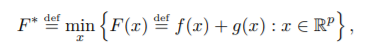
\includegraphics{min.png}
\caption{}
\end{figure}

\section{Métodos de primer orden}\label{metodos-de-primer-orden}

Cuando la función objetivo es suave, se asume como convexa y derivable,
para resolver este problema se utiliza el gradiente descendente y l
principio de mapeo próximo. son robustos para realizar optimizaciones y
son adecuados para computo paralelo. Este método utliza la siguiente
actualización en cada iteración \(k\): 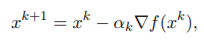
\includegraphics{soft.png}

aunque también existen otros métodos que son más rápidos como newton.

otro método es el de Nesterov:

\begin{figure}
\centering
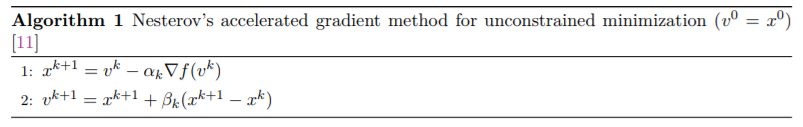
\includegraphics{nesterov.png}
\caption{}
\end{figure}

este es un método de primer orden óptimo que logra el menor error
posible en el peor escenario.

También existe el método del gradiente acelerado donde la función g
tiene la formulación de LASSO, si la función objetivo consiste en un
función convexa \(f\) y una función convexa no suave \(g\), en general
la no diferenciabilidad de \(g\) reduce la eficiencia de los métodos de
primer orden. No obstante, se pueden utilizar métodos de gradiente
proximales que utilizan la misma aproximación para \(f\) pero incluyen
el término g.

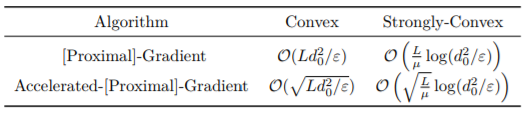
\includegraphics{acelerado.png} Número total de iteraciones soluciones
precisas de métodos de primer orden.

el operador proximal es eficiente y en otro caso particular donde g es
una función indicadora de un conjunto compacto, el problema de
optimización compuesto se pude resolver con el método de Frank-Wolfe:

\$\$ x\^{}\{k+1\} = prox\_\{\alpha\_k g\} * (v\^{}k - \alpha\_k *
\nabla{f(v^k)}) v\^{}\{k+1\} = x\^{}\{k+1\} + \beta\_k * (x\^{}\{k+1\} -
x\^{}k)

\$\$ \#Objetivos compuestos.

El objetivo \(F\) consiste de funciones \(f\) diferenciables y una
función no suavizada convexa \(g\). Los métodos de gradientes proximales
aprovechan la estructura compuesta para retener las mismas razones del
método gradiente para las clases de problema suave.

método acelerado de gradiente proximal:

\begin{figure}
\centering
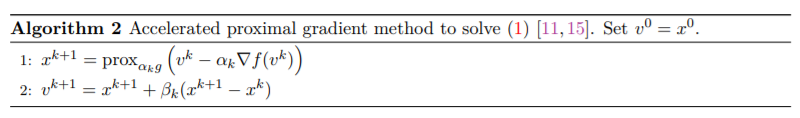
\includegraphics{prox.png}
\caption{}
\end{figure}

Algoritmo ADMM que utiliza técnicas Lagrangiana y descomposición dual:

\begin{figure}
\centering
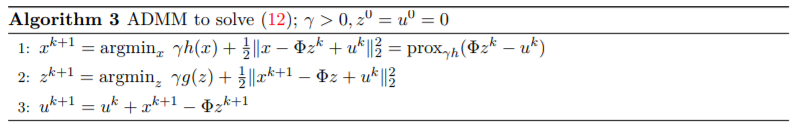
\includegraphics{admm.png}
\caption{}
\end{figure}

alternating direction method model, este algorimo es altamente
recomendable para optimización distribuida y requiere un parámetro de
penalización. 2 puntos en contra pues una parte del mismo se tiene que
resolver numéricamente y la otra es que si se realiza la extensión a
tener más dos términos objetivo, la convergencia ya no se está
garantizada.

\section{Aleatorización para la
escalabilidad}\label{aleatorizacion-para-la-escalabilidad}

En esta sección el artículo describe los métodos de descenso por
coordenada o entrada, metodos de gradiente estocástico y aleatoriedad en
algebra lineal.

En teoría, los métodos de primer orden están bien posicionados para
abordar problemas a gran escala. En la práctica, sin embargo, los
cálculos numéricos exactos que exigen sus iteraciones pueden hacer que
incluso estos métodos simples no factibles a medida que crecen las
dimensiones del problema.

\section{Descenso coordinado}\label{descenso-coordinado}

El cálculo del gradiente completo para la formulación del problema del
PageRank requiere una operación matriz-vector en cada iteración. Una
operación de vector más económica sería elegir una coordenada i de x y
solo modificar la variable correspondiente xi para mejorar la función
objetivo.

\begin{figure}
\centering
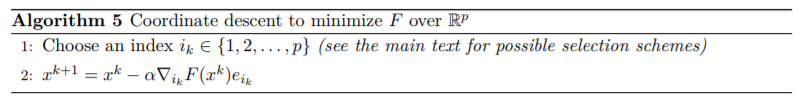
\includegraphics{coord.png}
\caption{}
\end{figure}

El ejemplo anterior subraya la dificultad fundamental en los métodos de
descendencia coordinada. Encontrar la mejor coordenada para actualizar,
el máximo de las magnitudes del elemento de degradado, puede requerir un
esfuerzo computacional tan alto como el cálculo del gradiente en sí
mismo.

\section{Métodos de gradiente
estocástico.}\label{metodos-de-gradiente-estocastico.}

\begin{figure}
\centering
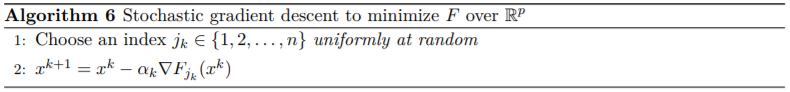
\includegraphics{alg6.png}
\caption{}
\end{figure}

En contraste con los métodos de coordenadas aleatorias, que actualizan
una sola coordenada a la vez con su gradiente exacto, los métodos de
gradiente estocástico actualizan todas las coordenadas simultáneamente
pero usan gradientes aproximados.

De forma similar a los métodos de descendencia coordinada, el problema
de diseño crucial en los métodos de gradiente estocásticos es la
selección de los puntos de datos j en cada iteración. Análogamente,
obtenemos mejores tasas de convergencia seleccionando j de manera
uniforme al azar en lugar de recorrer los datos.

\section{Algebra Lineal Aleatorizada}\label{algebra-lineal-aleatorizada}

En el caso de los problemas de Big Data, las operaciones de álgebra
lineal básica, como las descomposiciones de la matriz (por ejemplo,
valor propio, valor singular y Cholesky) y las multiplicaciones de
matrices y matrices pueden ser de gran importancia computacional.
cuellos de botella debido a su dependencia superlineal de las
dimensiones. Sin embargo, cuando la matriz relevante los objetos tienen
representaciones de bajo rango, a eficiencia de estos métodos mejora de
manera uniforme. Por ejemplo, el valor singular correspondiente la
descomposición (SVD) de M solo costaría fracasos O (pr 2 + r 3). La idea
detrás de los métodos de álgebra lineal aleatorizados es aproximar M ≈ Q
(Q T M) con Q ∈ R p × r, o para construir una representación de bajo
rango por selección de subconjunto de columna o fila en orden para
acelerar el cálculo.

Los impactos de este método son: acelerar el cómputo de operadores de
proximidad de funciones que dependen de valores espectrales de una
matriz, obtener gradiente no sesgado cuando la aleatorización es
seleccionada apropiadamente y Acercamiento aleatorizado puede ser
utilizado para realizar un bosquejo de funciones objetivo.

\section{Cómputo paralelo y
distribuido}\label{computo-paralelo-y-distribuido}

2 dificultades:

1.-Comunicación: los enlaces de comunicación desiguales o defectuosos
entre las computadoras y dentro de la jerarquía de la memoria local
pueden reducir significativamente la eficiencia numérica general de los
métodos de primer orden. Dos enfoques abordan ampliamente tales
inconvenientes. Primero, podemos diseñar específicamente algoritmos que
minimizan la comunicación. En segundo lugar, podemos eliminar un vector
maestro \(x_k\) y en su lugar, trabaje con una copia local en cada
máquina que conduzca a un consenso x? en la convergencia.

2.-Sincronización: para realizar exactamente los cálculos de forma
distribuida, primer orden los métodos deben coordinar las actividades de
diferentes computadoras cuyas primitivas numéricas dependen del mismo
vector \(x_k\) en cada iteración. Sin embargo, este procedimiento se
ralentiza incluso cuando una sola máquina lleva mucho más tiempo que las
otras. Para aliviar este problema de sincronización por excelencia, los
algoritmos asíncronos permiten actualizaciones utilizando versiones
obsoletas de sus parámetros

\section{Métodos asíncronos de primer orden con comunicaciones
descentralizadas}\label{metodos-asincronos-de-primer-orden-con-comunicaciones-descentralizadas}

El gradiente y los métodos de descomposición anteriores aún requieren
una sincronización global para manejar problemas. Por ejemplo, el
algoritmo de gradiente calcula el gradiente exactamente con respecto a
uno (o más) ejemplos en \(x_k\) y luego se sincroniza en secuencia para
actualizar \(x_{k + 1}\) en una implementación estándar. Por el
contrario, algoritmos de gradiente estocásticos que abordan solo usan
una aproximación cruda del gradiente. Por lo tanto, esperamos que este
algoritmo sea robusto.

\section{Métodos de primer orden con comunicaciones reducidas o
descentralizadas}\label{metodos-de-primer-orden-con-comunicaciones-reducidas-o-descentralizadas}

En sistemas grandes, comunicar el gradiente o sus elementos a una
ubicación central puede crear un cuello de botella en la comunicación.
En esta configuración, los métodos de descendencia coordinada
proporcionan un enfoque basado en principios para reducir las
comunicaciones. De hecho, hay un trabajo sustancial en el desarrollo de
versiones paralelas de estos métodos, que datan del trabajo sobre el
algoritmo de Jacobi para resolver sistemas lineales. La idea básica es
simplemente aplicar varias actualizaciones de descenso coordinado al
mismo tiempo en paralelo. La ventaja de esta estrategia en términos de
comunicación es que cada procesador solo necesita comunicar una única
actualización de coordenadas, mientras que solo necesita recibir las
actualizaciones de las coordenadas.

\section{Métodos de primer orden
paralelos}\label{metodos-de-primer-orden-paralelos}

En el cómputo paralelo, la formulación del problema convexo hace una
gran diferencia. Un importante ejemplo paralelo es el cálculo del vector
gradiente cuando el objetivo se descompone naturalmente. Aquí, podemos
procesar cada \(F_i\) con una de m computadoras usando solo
\(O (n / m)\) cómputo local. Cada máquina también almacena datos
localmente con las muestras de datos \(O (n / m)\) correspondientes, ya
que cada \(F_i\) corresponde directamente a un punto de datos. Cada
procesador entonces se comunica con la ubicación central para formar el
gradiente final y lograr el ideal lineal acelerar.

Los problemas de Big Data requieren una revisión fundamental de cómo
diseñamos algoritmos de optimización convexos y sugieren opciones
computacionales no convencionales. Este artículo deja en claro que
debemos identificar intercambios de aproximaciones algorítmicas
dependientes de la estructura clave. Dado que las limitaciones de
sincronización y comunicación del hardware disponible naturalmente dicta
la elección de los algoritmos, esperamos que las nuevas herramientas de
aproximación se adapten a los algoritmos convexos a la heterogeneidad de
las plataformas computacionales.

obtener la misma información, pero hacerlo más rápido, es un problema
que ha sido discutido pero aún no ha tenido impacto en la práctica.


\end{document}
